
\subsection[]{}
%___________________________________________________________________________________________________

\begin{frame}{Teilchendetektoren}
	\begin{description}
	  \item[Teilchendetektoren] Dienen dem Nachweis freier Teilchen durch Messung
	  verschiedener Parameter
	\end{description}
	
	\begin{block}{Häufig gemessene Eigenschaften}
		\begin{itemize}\setlength{\itemsep}{+5pt}
		  \item Geschwindigkeit
		  \item Impuls
		  \item Energie
		  \item Trajektorie
		  \item Zeit (Synchronisierung mit anderen Detektoren)
		  \item Ladung
		\end{itemize}
	\end{block}
\end{frame}

%___________________________________________________________________________________________________

	\begin{frame}{Spurdetektoren}
	\begin{description}
	  \item[Spurdetektoren] Bestimmen die Trajektorie eines Teilchens durch
	  Detektion an verschiedenen Orten und anschließender Rekonstruktion der
	  Bahnkurve
	\end{description}
	\begin{block}{Wozu die Trajektorie bestimmen?}
		\begin{itemize}\setlength{\itemsep}{+5pt}
		  \item Ursprung des Teilchens zurückverfolgen
		  	\begin{itemize}\setlength{\itemsep}{+5pt}
		    	\item Stammt Teilchen vom
		    	Kollisionspunkt$\rightarrow$Untergrundunterdrückung
		  	\end{itemize}
		  	\item \includesvg[svgpath=bilder/, width=5.7cm]{zerfallsstrecke}
		  	\item Messungen in Kombination mit Magnetfeld:
		   		\begin{itemize}\setlength{\itemsep}{+5pt}
		    		\item Ladung
		    		\item Impuls
		  		\end{itemize}
		\end{itemize}
	\end{block}
\end{frame}


\begin{frame}{Lorentzkraft}
	\begin{block}{Kraft auf geladene Teilchen bei magnetischer Flussdichte
	$\vec{B}$}
		$\vec{F}_L = q \cdot (\vec{v} \times \vec{B})$
	\end{block}
	\begin{block}{$\vec{F}_L$ führt zu Kreisbahn mit radius $r$}
		\begin{itemize}\setlength{\itemsep}{+5pt}
		  \item $r = \frac{m \cdot v}{q \cdot B} \propto \frac{p}{q}$
		  \item Vorzeichen der Krümmung ergibt Vorzeichen der Ladung $q$
		\end{itemize}
	\end{block}
	\begin{exampleblock}{Häufig ist Ladung erlaubter Sekundärteilchen eingeschränkt}
		$q \in \{- e, 0, +e\}$
		$\Rightarrow p = \pm e \cdot r \cdot B$
	\end{exampleblock}
\end{frame}
%___________________________________________________________________________________________________
%___________________________________________________________________________________________________

\subsection[]{}

%___________________________________________________________________________________________________

\begin{frame}{Pile-Up}
	An LHC-Experimenten wie ATLAS werden zukünftig alle 25 ns ca. 50
	Proton-Proton-Kollisionen gleichzeitig gemessen
	% http://iopscience.iop.org/1742-6596/513/2/022024/pdf/1742-6596_513_2_022024.pdf
	\begin{figure}[htp]
	\begin{center}
	  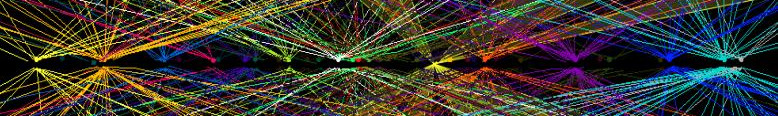
\includegraphics[width=\textwidth]{pileup.jpg}
	  \caption{Simulierter Pile-Up am CMS Detektor [cpu]}
	\end{center}
	\end{figure}
	\vspace{-0.7cm}
	\begin{block}{Jede Kollision muss isoliert analysiert werden (E- und
	p-Erhaltung)} Sekundärteilchen müssen je einer p-p-Kollision zugewiesen werden 
	\end{block}
	\begin{exampleblock}{Spurrekonstruktion nahe der Kollision}
		Schnittpunkt zwischen rekonstruierter Spur und Strahl stellt Ort der Kollision
		dar
	\end{exampleblock}
\end{frame}

%___________________________________________________________________________________________________


